\documentclass[a4paper,12pt]{article}
\usepackage[T2A]{fontenc}
\usepackage[utf8]{inputenc}
\usepackage[english,russian]{babel}
\usepackage[margin=2cm]{geometry}
\usepackage{fancyvrb}
\usepackage{inconsolata}
\usepackage{graphicx}

\newcommand\userinput[1]{\textbf{#1}}

\newcounter{problemnumber}

\newenvironment{problem}[1]
	{\addtocounter{problemnumber}{1}\arabic{problemnumber}. (#1)}
	{\vspace{6pt}}

\title{Домашняя работа 25}
\date{}
\begin{document}
\maketitle{}

\emph{Во всех программах размер экрана $640 \times 480$. Эти числа должны
    задаваться в виде констант в начале программы.}

\begin{problem}{Культин, 205}
    Написать программу, которая рисует на экране весёлую рожицу жёлтого цвета,
    как показано на рис.~\ref{fig:kultin205}.
\end{problem}

\begin{problem}{Культин, 209}
    Написать программу, которая выводит узор, как показано
    на рис.~\ref{fig:kultin209}.
\end{problem}

\begin{problem}{Культин, 210}
    Написать программу, которая выводит узор, изображённый
    на рис.~\ref{fig:kultin210}.
\end{problem}

\begin{figure}
    \centering
    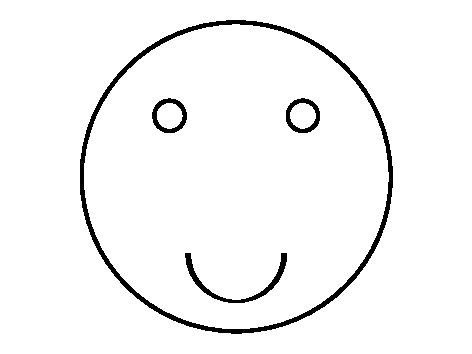
\includegraphics{kultin205}
    \caption{Иллюстрация к задаче 1.}
    \label{fig:kultin205}
\end{figure}

\begin{figure}
\centering
\begin{minipage}{.5\textwidth}
  \centering
  \includegraphics{kultin209}
  \caption{Иллюстрация к задаче 2.}
  \label{fig:kultin209}
\end{minipage}\hfill
\begin{minipage}{.5\textwidth}
  \centering
  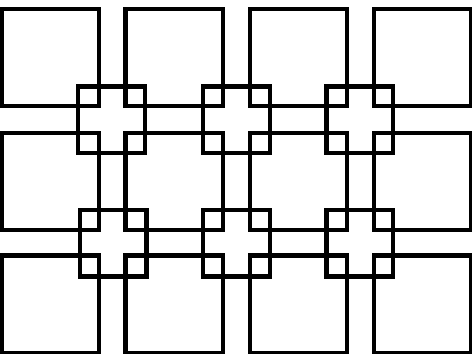
\includegraphics{kultin210}
  \caption{Иллюстрация к задаче 3.}
  \label{fig:kultin210}
\end{minipage}
\end{figure}

\end{document}
